\section{Back-End}
Jose I. Retamal
\vskip 0.1in
\indent
\indent

\subsection{Implementation}


The system is implemented using  6 Virtual machines( 2 in Azure, 1 in  AWS and 3 in gCloud), one file bucket(gCloud), and the React Native app Accessible through Google Play Store(Figure \ref{se:implementation}).

\begin{figure}[]
	\begin{center}
		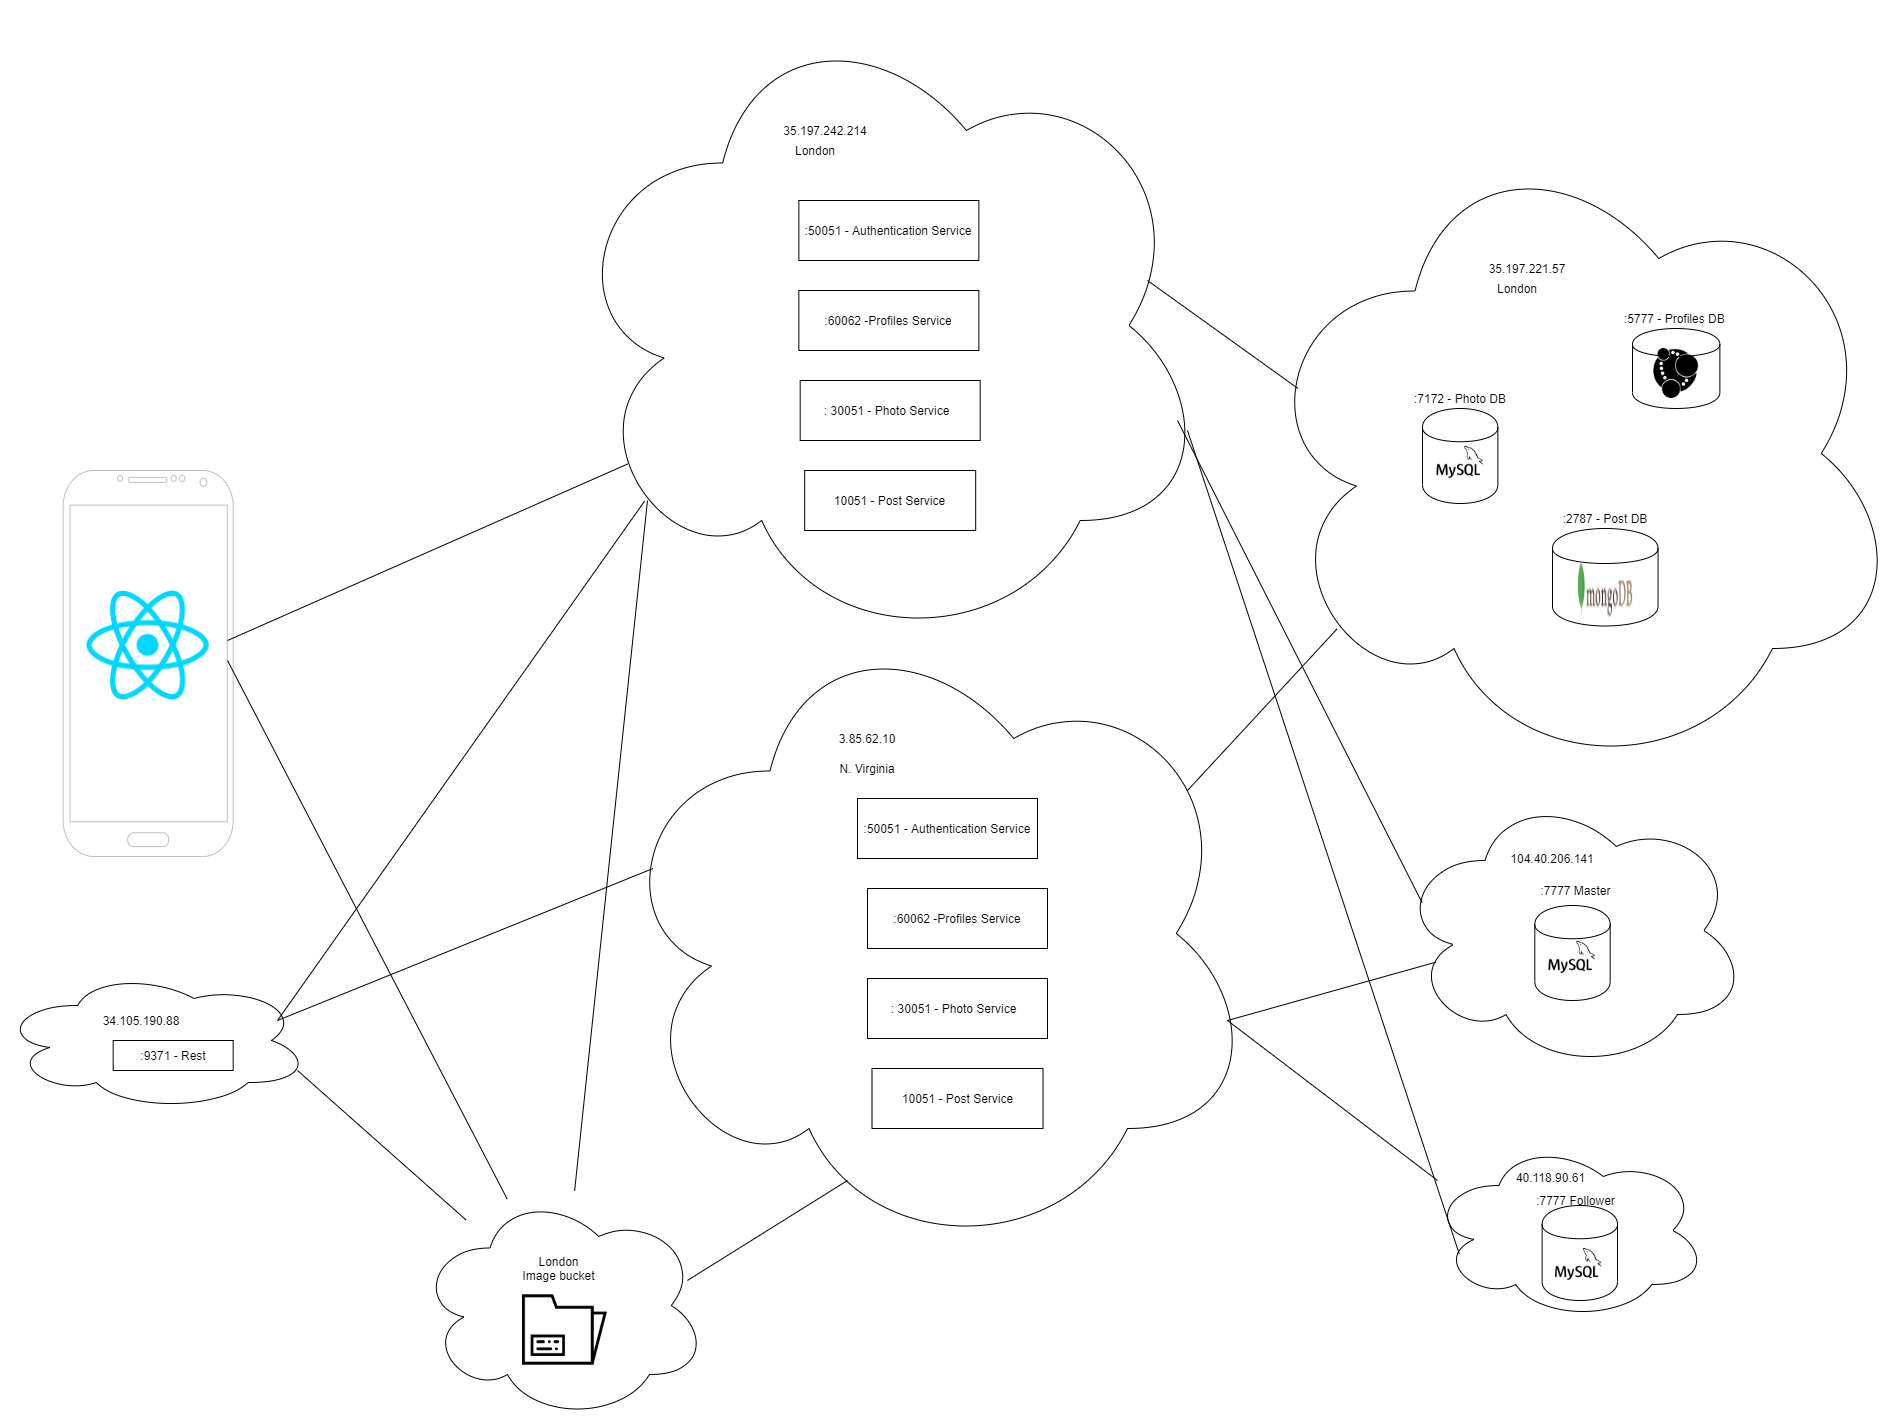
\includegraphics[width=120mm,scale=1]{img/implementation/VM-Diagram.png}
		\caption{System Implementation.}
		\label{se:implementation}
	\end{center}
	
\end{figure}

\subsubsection{The databases}

All databases are static, and they can be replicated or partitioned for scalability if we create multiple instances of one service, each instance access the same database or a replica of it. We have test replication in the authentication MySQL database. 





\paragraph{Profiles, posts and Photo databases}
\indent

For convenience and limitation of resources, the profiles neo4j database, post mongo database, and photos MySQL database run all in the same Virtual Machine.
\\

We implement them in a Google Cloud small  size VM:
\\
\indent

Ram: 1.7 GiB
\\
\indent
VCPU: 1
\\
\indent
Estimate cost: 14.04 p/month
\\
\indent
OS: Ubuntu Server 18.04 LTS Minimal
\\
\indent
Disk: Standard HHD
\\
\indent
Location: London
\\
\\
The Memory usage is show below (Figure \ref{se:d1}):
\begin{figure}[H]
	\begin{center}
		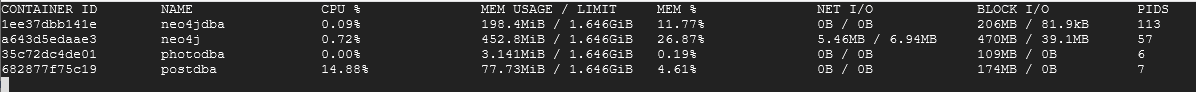
\includegraphics[width=170mm,scale=1]{img/implementation/databases-dock-stats.png}
		\caption{System Implementation: Databases Memory Usage.}
		\label{se:d1}
	\end{center}
	
\end{figure}

\paragraph{Auth database}
\indent
We have implemented one master and one follower, and each database runs in different virtual machines from Azure with same specifications, the VM speficcations are : 
\\
\indent
Ram: 1 GiB
\\
\indent
VCPU: 1
\\
\indent
Estimate cost: 6.96 p/month
\\
\indent
OS: Ubuntu Server 16.04 LTS
\\
\indent
Disk: Standard HHD
\\
\indent
Location: Western Europe

\begin{figure}[H]
	\begin{center}
		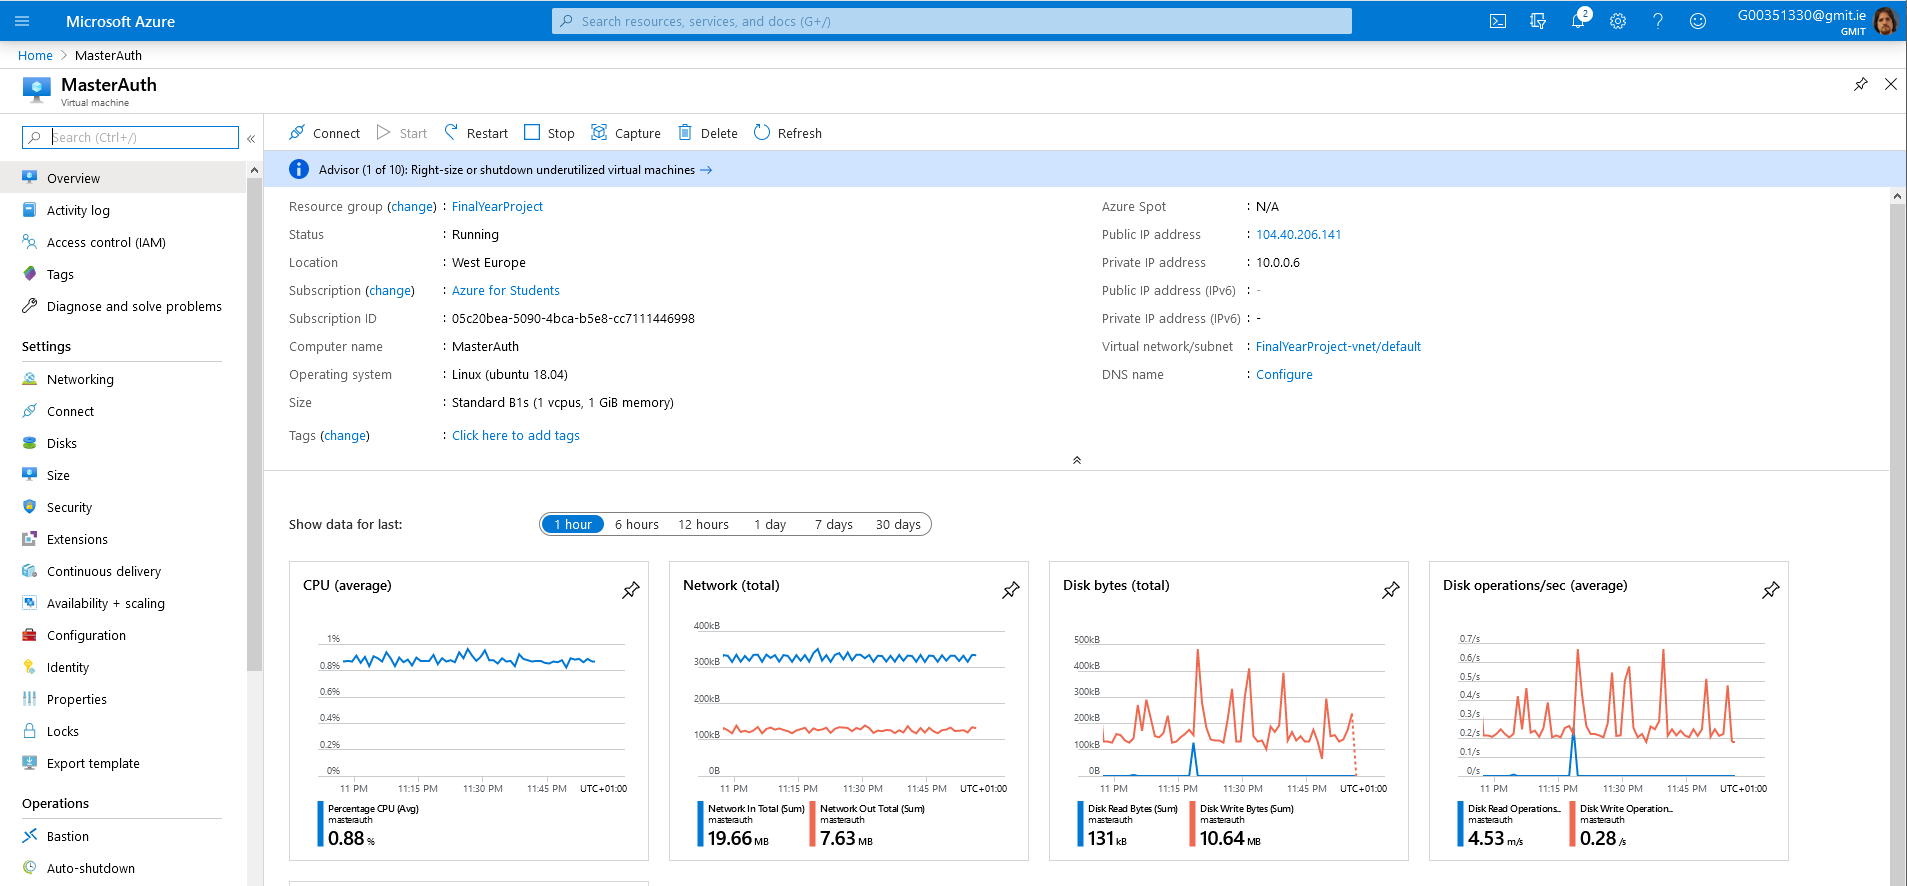
\includegraphics[width=170mm,scale=1]{img/implementation/auth-master-vm.png}
		\caption{System Implementation-Master VM.}
		\label{se:d2}
	\end{center}
	
\end{figure}

The memory usage for the master(Figure \ref{s2:d3}) :
\begin{figure}[H]
	\begin{center}
		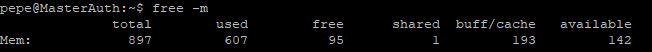
\includegraphics[width=170mm,scale=1]{img/implementation/auth-master-memory.png}
		\caption{System Implementation- Master Memory Usage.}
		\label{se:d3}
	\end{center}
	
\end{figure}
\indent
\paragraph{The Services}

Services need a small number of resources to run. The go service has a very low memory usage, and we were able to run all of them in a small virtual machine. We run on this way for testing and because we do not have many resources available to run the project.
We run two instances of each service, one in google cloud located in London(Figure \ref{s2d4}) and another in AWS in North Virginia(Figure \ref{s2:d5}).
\\
\indent
\subparagraph{Gcloud}

\indent
Ram: 0.6 GiB
\\
\indent
VCPU: 1
\\
\indent
Estimate cost: 5.39 p/month
\\
\indent
OS: Container Optimazed OS 69-10895.385.0 stable
\\
\indent
kernel :ChromiumOS-4.14.145 Kubernetes: 1.11.8 Docker: 17.03.2 Family: cos-69-lts 
\\
\indent
Disk: SSD
\\
\indent
Location: Western Europe

\begin{figure}[H]
	\begin{center}
		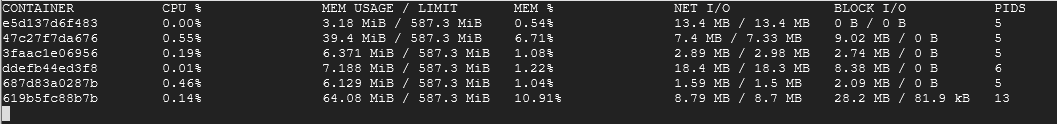
\includegraphics[width=170mm,scale=1]{img/implementation/gc-ser-stats.png}
		\caption{System Implementation- GCloun Services.}
		\label{se:d4}
	\end{center}
	
\end{figure}

\subparagraph{AWS}
\indent

Ram : 1 Gib
\\
\indent
VCPU : 1
\\
\indent
Esitmate Cost 3.97 p/month
\\
\indent
OS : ubuntu-bionic-18.04-amd64-server-20200112 
\\
\indent
Disk : Standard HHD
\\
\indent
Location: N. Virginia
\\
\begin{figure}[H]
	\begin{center}
		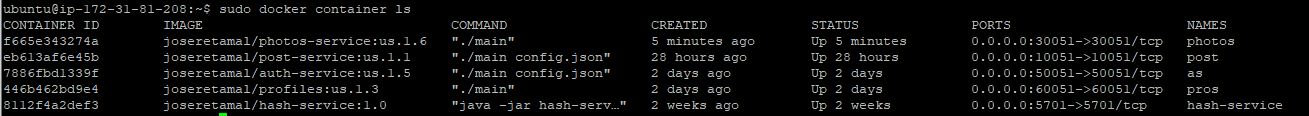
\includegraphics[width=170mm,scale=1]{img/implementation/was-service-ls.png}
		\caption{System Implementation- AWS Services.}
		\label{se:d5}
	\end{center}
	
\end{figure}
\paragraph{Rest service}
\indent
We run the rest service in a small VM on google cloud.
\subparagraph{Gcloud}

\indent
Ram: 0.6 GiB
\\
\indent
VCPU: 1
\\
\indent
Estimate cost: 5.39 p/month
\\
\indent
OS: Container Optimazed OS 69-10895.385.0 stable
\\
\indent
kernel :ChromiumOS-4.14.145 Kubernetes: 1.11.8 Docker: 17.03.2 Family: cos-69-lts 
\\
\indent
Disk: SSD
\\
\indent
Location: Western Europe


\subsection{REST API}
\vskip 0.1in
\indent
\indent
The rest API get data from all the services and create a JSON response. 

The rest API test all services; they perform fine, and the response time is quick. It uses two clusters to balance the request.
We use postman to test the API; this is the outcome:

\begin{itemize}


	\item  All request serves in less than a second even when they are done in a server in N. Virginia.
	\item  Security tokens are always validated. If the token is not valid, request are refused.
	\item  If one cluster is down, the request goes automatically to the other. This is a gRPC load balancer feature.
\end{itemize}

\paragraph{JSON response from  city Profile}

\begin{minted}[linenos,tabsize=2,breaklines]{JSON}
{
	"Name": "galway",
	"Country": "ireland",
	"CreatorEmail": "g00351330@gmit.ie",
	"Location": {
	"lon": 90,
	"lat": 89
	},
	"Description": "Galway is renowned for its vibrant lifestyle and for hosting numerous festivals, celebrations and events[4] such as The Galway Arts Festival. In 2018, it was named the European Region of Gastronomy.[citation needed] The city is currently the European Capital of Culture for 2020, alongside Rijeka, Croatia. ",
	"Images": [
	{
		"id": 86,
		"cityId": 212,
		"url": "https://storage.googleapis.com/wcity-images-1/city-1/1294648_1194511.jpg",
		"timestamp": "2020-05-09 21:05:21"
	}
	],
	"Posts": [
	{
		"CreatorEmail": "g00351330@gmit.ie",
		"Title": "Sunny day in Galway",
		"Body": "This is weird.",
		"TimeStamp": "UnixDate",
		"MongoId": "5eb70f3bfd2fed23c2eb899f",
		"ImageURL": "https://storage.googleapis.com/wcity-images-1/post-1/1474622_1764929.jpg"
	},
	{
		"CreatorEmail": "g00351330@gmit.ie",
		"Title": "Nice view of GAlway docks",
		"Body": "In my friend house",
		"TimeStamp": "UnixDate",
		"MongoId": "5eb70f69fd2fed23c2eb89a0",
		"ImageURL": "https://storage.googleapis.com/wcity-images-1/post-1/1629109_1282408.jpg"
	}
	],
	"Places": [
	{
		"PlaceId": 215,
		"Name": "gmit",
		"City": "galway",
		"Location": {
		"lon": 90,
		"lat": 89
		},
		"Description": "Institute of Technologies",
		"Images": [
			{
			"id": 192,
			"placeId": 215,
			"url": "https://storage.googleapis.com/wcity-images-1/place-1/1713341_1425286.jpg",
			"timestamp": "2020-05-09 21:10:03"
			}
		]
		},
		{
		"PlaceId": 214,
		"Name": "shop street",
		"City": "galway",
		"Location": {
		"lon": 90,
		"lat": 89
		},
		"Description": "Main pedistrian street in galway",
		"Images": [
			{
			"id": 191,
			"placeId": 214,
			"url": "https://storage.googleapis.com/wcity-images-1/place-1/1566362_1091161.jpg",
			"timestamp": "2020-05-09 21:09:06"
			}
	]
	}
	]
}
\end{minted}




\paragraph{JSON response from  user Profile}

\begin{minted}[linenos,tabsize=2,breaklines]{JSON}
{
	"Email": "g00351330@gmit.ie",
	"Name": "jose",
	"Descripiton": "Student",
	"Avatar": [
		{
		"id": 29,
		"userEmail": "g00351330@gmit.ie",
		"url": "https://storage.googleapis.com/wcity-images-1/profile-1/1317523_1625526.jpg",
		"timestamp": "2020-05-09 21:06:03",
		"selected": true
		}
	],
	"VisitedCities": [
		{
		"CityId": 212,
		"Name": "galway",
		"Country": "ireland",
		"CreatorEmail": "g00351330@gmit.ie",
		"Description": "Galway is renowned for its vibrant lifestyle and for hosting numerous festivals, celebrations and events[4] such as The Galway Arts Festival. In 2018, it was named the European Region of Gastronomy.[citation needed] The city is currently the European Capital of Culture for 2020, alongside Rijeka, Croatia. ",
		"Location": {},
		"Images": [
		{
		"id": 86,
		"cityId": 212,
		"url": "https://storage.googleapis.com/wcity-images-1/city-1/1294648_1194511.jpg",
		"timestamp": "2020-05-09 21:05:21"
		}
		]
		},
		{
		"CityId": 212,
		"Name": "galway",
		"Country": "ireland",
		"CreatorEmail": "g00351330@gmit.ie",
		"Description": "Galway is renowned for its vibrant lifestyle and for hosting numerous festivals, celebrations and events[4] such as The Galway Arts Festival. In 2018, it was named the European Region of Gastronomy.[citation needed] The city is currently the European Capital of Culture for 2020, alongside Rijeka, Croatia. ",
		"Location": {},
		"Images": [
		{
		"id": 86,
		"cityId": 212,
		"url": "https://storage.googleapis.com/wcity-images-1/city-1/1294648_1194511.jpg",
		"timestamp": "2020-05-09 21:05:21"
		}
		]
		}
	],
	"VisitedPlaces": [
		{
			"PlaceId": 214,
			"Name": "shop street",
			"City": "galway",
			"Country": "ireland",
			"Location": {
			"lon": 90,
			"lat": 89
		},
		"Description": "Main pedistrian street in galway",
		"Images": [
		{
		"id": 191,
		"placeId": 214,
		"url": "https://storage.googleapis.com/wcity-images-1/place-1/1566362_1091161.jpg",
		"timestamp": "2020-05-09 21:09:06"
		}
		]
		},
		{
			"PlaceId": 215,
			"Name": "gmit",
			"City": "galway",
			"Country": "ireland",
			"Location": {
			"lon": 90,
			"lat": 89
		},
			"Description": "Institute of Technologies",
			"Images": [
			{
			"id": 192,
			"placeId": 215,
			"url": "https://storage.googleapis.com/wcity-images-1/place-1/1713341_1425286.jpg",
			"timestamp": "2020-05-09 21:10:03"
		}
	]
	}
	]
}
\end{minted}